\chapter{Rotationel Mekanik}
Legemers bevægelse kan, i den newtonske mekanik, groft sagt deles op i to kategorier - translatorisk og rotationel bevægelse, hvilket vil sige bevægelse med og uden rotation. Vi skal se på den roterende del af legemers bevægelse, hvor der vil fokuseres på stive legemer, da de er lettest at behandle. Beskrivelsen af roterende legemer deles op i tre dele - kinematik, energi og dynamik. Kinematik er beskrivelsen af legemers bevægelse, og her stilles ikke spørgsmålstegn ved bevægelsens oprindelse, men der forsøges at opnå en beskrivelse af en bevægelse med en matematisk model. Dynamik beskriver hvorfor ting bevæger sig, som de gør, og energi er en vigtig faktor i disse betragtninger. For at få en god forståelse for dynamik er vektorregningen essentiel, ligesom differentialregningen er vigtig for kinematikken, hvorfor det vil være en god ide at have læst appendikset om disse to emner.

\section{Kinematik}
I den translatoriske bevægelse beskrives et legemes position ved kartesiske koordinater $(x,y,z)$, der udgør et koordinatsystem, som I kender det. Ud fra disse, defineres hastighed, $\v{v}$, og acceleration, $\v{a}$, som
\begin{equation}
    \v{v} \equiv \d{\v{x}}{t} \qquad \v{a} \equiv \dd{\v{x}}{t}
\end{equation}
Den gennemsnitlige hastighed for et legeme over et tidsrum er så
\begin{equation}
    \v{v}_{\text{av}} = \frac{\v{x}_2-\v{x}_1}{t_2-t_1}
\end{equation}
\begin{figure}[h!]
\centering
\includegraphics[width=.35\textwidth]{RotationelMekanik/CylindriskeKoordinater}
\caption{I det cylindriske koordinatsystem angives afstanden til $z$-aksen som første koordinat, samt forskydningen langs samme akse som $z$-koordinat. Derudover angives vinklen med polæraksen, her ækvivalent med $x$-aksen. $z$-koordinatet er derved det samme i det kartesiske og cylindriske koordinatsystem.}
\label{fig:CylindriskeKoordinater}
\end{figure}
hvor $\v{x}_i$ angiver legemets stedvektor til tiden $t_i$. Noget lignende gøres for legemers rotation, hvor der her kun fokuseres på rotation om én akse.

\subsubsection{Cylindriske Koordinater}
Til beskrivelsen af roterende legemer benyttes cylindriske koordinater i stedet for almindelige, kartesiske koordinater. Cylindriske koordinater er en tredimensionel udvidelse af de todimensionelle polære koordinater (se A.1), hvor 3. koordinatet, $z$, forskyder punktet parallelt med en akse, der er ortogonal på den todimensionelle plan udspændt af de polære koordinater, gennem origo, (0,0,0). I polære koordinater defineres et punkt  som origo, og udfra det, en polærakse, der angiver placeringen af vinklen på 0 radianer. Et punkts afstand til origo, $r$, og dets vinkel med polæraksen, $\theta$, angiver så de polære koordinater. Defineres koordinatsystemet således at polæraksen og $x$-aksen i et tilsvarende kartesisk koordinatsystem er sammenfaldende, ville $\theta$ være vinklen ift. polæraksen i $x,y$-planen og $z$ er forskydningen ift. polærplanen, se Figur \ref{fig:CylindriskeKoordinater}. Det bemærkes, at det kartesiske 3. koordinat og det cylindriske 3. koordinat er ens, og at afstanden $r$ ved udvidelsen fra polære til cylindriske koordinater bliver afstanden til $z$-aksen og ikke afstanden til origo. Da der kun fokuseres på legemers rotation om én akse, kan $z$-aksen defineres til at være denne rotationsakse, hvorved det cylindriske 3. koordinat forbliver uændret i tid.

\subsection{Vinkelhastighed og Acceleration}
\begin{figure}[h!]
\centering
\includegraphics[width=.3\textwidth]{RotationelMekanik/Roterende-Legeme}
\caption{ Til to forskellige tider har det blå punkt to forskellige vinkler med polæraksen (grå), der her er sammenfaldende med den kartesiske $x$-akse, mens legemet roterer om $z$-aksen. $\v{r}$ er en vektor fra origo til punktet, og har derfor længden $r$ og vinklen $\theta$ med polæraksen.}
\label{fig:Roterende-Legeme}
\end{figure}

Figur \ref{fig:Roterende-Legeme} viser hvordan vinklen $\theta$ ændrer sig fra tidspunktet $t_1$ til $t_2$. Helt analogt til den translatoriske bevægelse defineres vinkelhastigheden, $\omega$, og vinkelacceleration, $\alpha$, som
\begin{equation}
    \omega\equiv\d{\theta}{t} \qquad\qquad \alpha\equiv\d{\omega}{t}=\dd{\theta}{t}
\end{equation}
Vinkelhastigheden er et udtryk for, hvor hurtigt et legeme roterer og har enheden $\SI{}{\frac{\radian}{\second}}$. Vinkelaccelerationen udtrykker, hvor hurtigt rotationshastigheden ændres i $\SI{}{\frac{\radian}{\second\squared}}$. Her er "$\SI{}{\radian}$" symbolet for enheden radianer. \\

Legemer kan deles op i mange små elementer, kaldet delelementer, der eksempelvis kan tænkes som de individuelle træpartikler i et stykke træ. I dette eksempel omtales hele træstykket som legemet, mens træpartiklerne benævnes delelementer. Et stift legeme defineres nu, som værende et legeme, hvor alle delelementer har samme vinkelhastighed og samme vinkelacceleration, hvorfor der om et delelement, $i$, i et roterende legeme med vinkelhastighed $\omega$ gælder at
\begin{equation}
\omega_i = \omega \quad\forall\, i
\end{equation}
Med symbolet $\forall$ menes \textit{for alle}. Defineres $z$-aksen som værende rotationsaksen, vil $r_i$ være det $i$'te delelements afstand til rotationsaksen og $\theta_i$ bliver samme elements vinkel med polæraksen. For det $i$'te element eksisterer en sammenhæng mellem dets fart og det stive legemes vinkelhastighed, samt legemet vinkelacceleration og elementets tangentielle acceleration. Disse bliver
\begin{equation} \label{eq:Stift-Legeme}
    v_i=r_i\omega \qquad\qquad a_{\text{tan},\,i}=r_i\alpha
\end{equation}
Hastigheder og accelerationer, ligning \ref{eq:Stift-Legeme}, er ift. massemidtpunktet, også når legemer med bevægende massemidtpunkt beskrives. Massemidtpunktet er et vægtet gennemsnit af placeringerne af et legemes delelementer, hvor vægtningen er massen af delelementerne. Består et legeme af $n$ delelementer med masserne $m_i$, placeret i punkterne givet ved stedvektoren $\v{r}_i$, så er defintionen af massemidtpunktet
\begin{equation}
\v{r}_\text{cm} \equiv \dfrac{\sum\limits_i^nm_i\v{r}_i}{\sum\limits_i^nm_i}
\end{equation}
I det tilfælde bliver et elements totalhastighed vektorsummen af disse hastigheder. Hele legemets roterende bevægelse kan derfor beskrives ved dets vinkelhastighed og vinkelacceleration samt massemidtpunktets hastighed og acceleration. Det bemærkes, at det er den tangentielle acceleration, dvs. accelerationen i retningen givet af tangenten til punktets banekurve, der kan bestemmes ved ligning \ref{eq:Stift-Legeme}, og ikke elementets totale acceleration. Den radielle acceleration, altså accelerationen ind mod rotationsaksen, kan ved kombination af ligning \ref{eq:Stift-Legeme} og en kendt ligning fra jævn cirkelbevægelse, $a=\frac{v^2}{r}$, bestemmes som 
\begin{equation}
     a_{\text{rad},\,i} = \frac{v_i^2}{r_i} = \omega^2r_i
\end{equation}

\subsection{Inertimomentet}
Eksperimenter viser, at et legemes modstand mod acceleration ikke kun afhænger af legemets masse, men også placeringen af massen, hvorfor inertimomentet for et objekt defineres som
\begin{equation} \label{eq:Inertimoment}
    I \equiv \sum m_ir_i^2
\end{equation}
hvor $m_i$ er massen af det $i$'te masseelement og $r_i$ er samme masseelements afstand til rotationsaksen. Inertimomentet for et givet legeme udtrykker, hvor langt fra rotationsaksen et legemes masse er placeret, og det afhænger da af den akse, som legemet  roterer om.

\section{Energi}
For translatorisk bevægelse defineres kinetisk energi som
\begin{equation} \label{eq:Ktrans}
    K_{\text{trans}}=\frac{1}{2}mv_\text{cm}^2
\end{equation}
mens rotationskinetisk energi defineres som
\begin{equation} \label{eq:Krot}
    K_{\text{rot}}=\frac{1}{2}I\omega^2
\end{equation}
hvor den totale kinetiske energi for et roterende legeme er summen af de to ovenstående
\begin{equation} \label{eq:K}
    K_{\text{tot}}=K_{\text{trans}}+K_{\text{rot}}
\end{equation}
Dette kan vises ved først at definere massemidtpunktets hastighed
\begin{equation} \label{eq:v_cm}
    \v{v}_\text{cm}=\frac{\sum m_i\v{v}_i}{\sum m_i}
\end{equation}
Det skal med henblik på udledningen bemærkes at, der om summer gælder følgende
\begin{equation}
    \sum_i^n a_ic=c\sum_i^n a_i \qquad\qquad \sum_i^n\left(a_i + b_i\right) = \sum_i^n a_i + \sum_i^n b_i
\end{equation}
hvor $c$ er en størrelse, der er konstant for alle værdier af indekset $i$. $a_i$ og $b_i$ er størrelser, der afhænger af indekset $i$. \\

Et delelements hastighed, $\v{v}_i$, kan skrives som en sum af massemidtpunktets hastighed, $\v{v}_\text{cm}$, og elementets hastighed ift. massemidtpunktet, $\v{v}_i'$. Af definitionen for translatorisk kinetisk energi er det $i$'te delelementets kinetiske energi
\begin{equation}
     K_i=\frac{1}{2}m_i\v{v}_i^2=\frac{1}{2}m_i(\v{v}_\text{cm}^2+\v{v}_i'^2+2\v{v}_\text{cm}\v{v}_i')
\end{equation}
Den totale kinetiske energi bliver summen af de enkelte deles kinetiske energi
\begin{equation} \label{eq:Ktot}
    K_\text{tot} = \sum\frac{1}{2}m_i{\v{v}_\text{cm}}^2+\sum\frac{1}{2}m_i\v{v}_i'^2+\sum m_i\v{v}_\text{cm}\v{v}_i' = \frac{1}{2}{\v{v}_\text{cm}}^2\sum m_i+\frac{1}{2}\sum m_i\v{v}_i'^2+\v{v}_\text{cm}\sum m_i\v{v}_i'
\end{equation}
Da totalmassen af et legeme er summen af massen af de enkelte masseelementer, $M=\sum m_i$, er første led i ligning \ref{eq:Ktot} den totale translatoriske kinetiske energi for hele legemet, $K_\text{trans}$. \\
$\v{v}_i'$ er hastigheden ift. massemidtpunktet hvorved ligning \ref{eq:Stift-Legeme} gælder. Det medfører at
\begin{equation} \label{eq:K_rot}
     \frac{1}{2}\sum m_i\v{v}_i'^2=\frac{1}{2}\sum\left(m_ir_i^2\right)\omega^2=\frac{1}{2}I\omega^2 = K_\text{rot}
\end{equation}
Her er definitionen af inertimomentet, ligning \ref{eq:Inertimoment}, samt det faktum, at der kigges på et stift legeme, benyttet.\\
For at ligning \ref{eq:Krot} giver mening, skal det sidste led i ligning \ref{eq:K_rot} være nul for at opfylde ligning \ref{eq:K}. Det vises ved først at omskrive $\v{v}_i'$ i det sidste led i ligning \ref{eq:K_rot}
\begin{equation} \label{eq:v_i}
     \v{v}_i'=\v{v}_i-\v{v}_\text{cm}
\end{equation}
Multipliceres ligning \ref{eq:v_i} med $m_i$, hvorefter der summeres, opnås
\begin{equation} \label{eq:K3}
     \sum m_i(\v{v}_i-\v{v}_\text{cm}) = \sum m_i\v{v}_i-\v{v}_\text{cm}\sum m_i = \v{v}_\text{cm}\sum m_i - \v{v}_\text{cm}\sum m_i = \v{0}
\end{equation}
hvor ligning \ref{eq:v_cm} er benyttet. \\
Kombineres ligningerne \ref{eq:Ktot}, \ref{eq:K_rot} og \ref{eq:K3} får man
\begin{equation} \label{eq:KinetiskEnergi}
     K_\text{tot} = \frac{1}{2}M{v_{\text{cm}}}^2 + \frac{1}{2}I_{\text{cm}}\omega^2 + \v{v}_{\text{cm}} \cdot \v{0} = K_{\text{trans}} + K_{\text{rot}}
\end{equation}
hvor $I_\text{cm}$ er inertimomentet for rotationen om en akse gennem massemidtpunktet. Da ligningerne \ref{eq:Ktrans} og \ref{eq:Krot} opfylder ligning \ref{eq:K} giver definitionen af  rotationel kinetisk energi mening.

\subsection{Energibevarelse}
Energi er altid bevaret, såfremt et legeme kun påvirkes af konservative kræfter\footnote{En kraft hvis arbejde på en partikel under bevægelsen mellem to punkter er uafhængig af vejen mellem de to punkter.} er
\begin{equation} \label{eq:Energi}
    U_1 + K_1 = U_2 + K_2
\end{equation}
hvor $U_i$ er den potentielle energi for summen af de konservative kræfter, der påvirker legemet til tidspunktet $t_i$, og $K_i$ er legemets kinetiske energi til samme tidspunkt.

\subsubsection{Ruller uden at glide}
En nødvendig antagelse i forbindelse med mange problemer, der involverer rotation, er at friktionen mellem legemet og kontaktfladen er så stor, at legemet ruller uden at glide. Det punkt, hvor legemet rør kontaktfladen, er i hvile for at opfylde antagelsen, hvorfor farten fra ligning \ref{eq:Stift-Legeme} skal være ligestor og modsatrettet ift. massemidtpunktets hastighed, således at summen af disse bliver nul. Hvis legemet er cirkulært symmetrisk omkring rotationsaksen gælder der at
\begin{equation} \label{eq:RollingWithoutSlipping}
    v_\text{cm} = R\omega
\end{equation}
hvor $R$ er legemets radius. Det er specielt vigtigt, hvis rotationsaksen flytter sig i tid, da det er besværligt at behandle med dynamik. Det skyldes at kraftmomentet, som defineres nedenfor, er defineret ud fra rotationsaksen, hvorfor det bliver svært at bestemme og arbejde med. 

\section{Dynamik}
\begin{figure}[h!]
\centering
\includegraphics[width=.37\textwidth]{RotationelMekanik/Angrebspunkt}
\caption{En arbitrær kraft, $\v{F}$, virker i det røde punkt, hvorfor dette punkt kaldes kraftens angrebspunkt. Legemet roterer om en akse gennem det blå punkt, der er ortogonal på tegningen. Det blå punkt kan defineres som origo, hvorved vektoren fra rotationsaksen til kraftens angrebspunkt kaldes kraftens arm $\v{r}$. Kraftmomentet $\gv{\tau}$ peger ud af tegningen.}
\label{fig:Angrebspunkt}
\end{figure}
Kræfter er årsagen til bevægelse, som det kendes i fysik, og med hensyn til den translatoriske bevægelse, er det ikke essentielt, hvor på legemet kraften virker, men det er det for rotationel bevægelse. Der findes mange dagligdags eksempler på dette, hvor et af de bedre er et værktøj, som en svensknøgle, der holder om en bolt. Jo længere nede på svensknøglen man holder, desto lettere er det at stramme eller løsne bolten. For at forstå fysikken bag dette, introduceres angrebspunktet for kraften $\v{F}$ som det punkt på et legeme, hvorpå kraften virker, se Figur \ref{fig:Angrebspunkt}. Yderligere defineres en vektor til kraftens angrebspunkt, hvilket kaldes kraftens arm $\v{r}$. Dennes oprindelse defineres frit, men der ville ofte være punkter, der er oplagte at bruge som origo for det koordinatsystem, der benyttes i en given situation. Herved kan kraftmomentet, $\gv{\tau}$, defineres
\begin{equation} \label{eq:Kraftmoment}
    \gv{{\tau}} \equiv \v{r}\times\v{F}
\end{equation}
Kraftmomentet er en vektor, der står ortogonalt på både kraften og dens arm, og den er parallel med rotationaksen. Kraftmomentets størrelse kan bestemmes som
\begin{equation} \label{eq:KraftmomentNorm}
\tau = rF\sin\phi
\end{equation}
hvor $\phi$ er vinklen mellem $\v{r}$ og $\v{F}$.

\begin{figure}[h!]
\centering
\includegraphics[width=.22\textwidth]{RotationelMekanik/Stift-legeme}
\caption{Arbitrært stift legeme, hvor kraften, $\v{F}_i$, peger ind i tegningen, og kraftens arm, $\v{r}_i$, er defineret ud fra punktet $O$.}
\label{fig:Stift-legeme}
\end{figure}

\subsection{Newtons Anden Lov for Roterende Legemer}
Newtons anden lov siger, at $\sum\v{F}=m\v{a}$, og der ønskes en tilsvarende formel for legemers resulterende kraftmoment. Der kigges nu på kraftmomentet for den $i$'te partikel i et arbitræt stift legeme, se Figur \ref{fig:Stift-legeme}. \\
Det ses, at $\v{r}_i\perp\v{F}_i$, og $\v{F}_i$ antages til at være den resulterende kraft på den $i$'te partikel, hvorfor kraftmomentets størrelse, af ligning \ref{eq:Stift-Legeme} og ligning \ref{eq:KraftmomentNorm}, bliver
\begin{equation}
    \tau_i = r_iF_i\ = r_im_ia_i = r_im_iR_i\alpha
\end{equation}
hvor Newtons 2. lov også er brugt. $\theta$ defineres som værende vinklen mellem rotationsaksen og kraftens arm. Det ses i figur \ref{fig:Stift-legeme} at følgende sammenhæng gælder
\begin{equation}
    R_i=r_i\sin\theta
\end{equation}
Tegnes kraftmomentet associeret med $\v{F}_i$ og deles den op i en $x$- og $z$-komposant ses det at
\begin{align}
\tau_{i,z} = \tau_i\sin\theta
\end{align}
hvorved $z$-komposanten af kraftmomentet bliver
\begin{equation}
    \tau_{i,z}=m_iR_i^2\alpha_z
\end{equation}
Summeres disse komposanter af delelementernes resulterende kraftmoment fås
\begin{equation} \label{eq:N2R}
    \sum\tau_{i,z}=\alpha_z\sum m_iR_i^2=I_z\alpha_z
\end{equation}
hvor $I_z$ er legemets inertimoment ved rotation om rotationsaksen. \\
Hvis legemet er symmetrisk omkring den givne rotationsakse bliver
\begin{equation} \label{eq:N2Rot}
    \sum\gv{\tau}_{i}\parallel \zhat \quad\Rightarrow\quad \sum\tau_{i}=I_z\alpha_z
\end{equation}
Ligning \ref{eq:N2R} kaldes ofte for Newtons anden lov for rotationel bevægelse, og koordinatsystemet skal fastholdes under hele bevægelsen for, at ligningerne \ref{eq:N2R} og \ref{eq:N2Rot} gælder.

\begin{figure}[h!]
\centering
\includegraphics[width=.25\textwidth]{RotationelMekanik/Impulsmoment}
\caption{ Det $i$'te delelement af et arbitrær stift legeme, med hastighed og impulsmoment som vist, hvor kraftens arm er defineret ud fra et punkt på rotationsaksen.}
\label{fig:Impulsmoment}
\end{figure}

\subsection{Impulsmoment}
Impulsmomentet, $\v{L}$, er bevaret, hvis summen af kraftmomenter er nul og af definitionen på impuls, $\v{p}$, er det logisk at definere impulsmomentet som
\begin{equation} \label{eq:L}
    \v{L} \equiv \v{r}\times\v{p}, \quad \v{p} \equiv m\v{v}
\end{equation}
Størrelsen på kraftmomentet er
\begin{equation}
L=rp\sin\theta
\end{equation}
hvor $\theta$ er vinklen mellem $\v{r}$ og $\v{p}$. Differentieres ligning \ref{eq:L} med hensyn til tiden fås
\begin{equation}
    \d{\v{L}}{t} = \d{}{t}\left(\v{r}\times\v{p}\right) = \d{\v{r}}{t}\times m\v{v}+\v{r}\times m\d{\v{v}}{t} = \v{v}\times m\v{v}+\v{r}\times m\v{a} = \v{r}\times\sum\v{F} = \sum\gv{\tau}
\end{equation}
idet et vektorpordukt af to parallelle vektorer er nul. Det er da vist at
\begin{equation}
    \sum\gv{\tau} = \d{\v{L}}{t}
\end{equation}
Det kan vises at summen af de indre kraftmomenter er nul, og impulsmomentet er da bevaret, hvis og kun hvis summen af de ydre kraftmomenter er nul. \\

For et stift legeme, der ikke er påvirket af nogle ydre kraftmomenter, som vist i Figur \ref{fig:Impulsmoment}, er
\begin{equation} \label{eq:Arm}
    \v{r}_i\perp\v{v}_i \quad\text{og}\quad R_i=r_i\sin\theta
\end{equation}
hvorfor det $i$'te elements impulsmoment, af ligning \ref{eq:Stift-Legeme}, bliver
\begin{equation} \label{eq:Impulsmoment}
    L_{i} = r_im_iv_i = r_im_iR_i\omega_z
\end{equation}
$z$-komposanten af impulsmomentet for $i$ er bevaret, da delelementet ikke påvirkes af nogle ydre kraftmomenter, mens de to andre komposanter ændres i tid. Derved giver ligningerne \ref{eq:Arm} og \ref{eq:Impulsmoment}
\begin{equation}
     L_{z,i}=L_i\sin\theta=r_im_iv_i\sin\theta=m_iR_i^2\omega_z
\end{equation}
Summeres nu over alle legemets partikler opnås
\begin{equation}
    \sum L_{z,i}=\sum m_iR_i^2\omega=I_z\omega_z
\end{equation}
Hvis legemet er symmetrisk omkring rotationsaksen, vil der være et punkt, hvis $x$- og $y$-komposanter af impulsmomentet går ud med det oprindelige punkts. Ergo bliver summen af impulsmomenter parallel med $z$-aksen
\begin{equation}
    \sum\v{L}_i = I_z\gv{\omega}
\end{equation}

\section{Løsning af Fysiske Problemstillingerne}
Fysiske problemstillinger kan løser på flere måder afhængig af problemet. Her vil nogle løsningsstrategier for forskellige fysiske problemstillinger vises.

\subsection{Energibetragtninger}
En cylinder ruller ned af et skråplan fra hvile, og det ønskes at bestemme cylinderens hastighed i bunden af skråplanet. Her er energibevarelse en oplagt løsningsstrategi, da cylinderen accelereres af tyngdekraften, der er en konservativ kraft. Antages det, at cylinderen "ruller uden at glide"  tabes intet energi til friktion mellem skråplanet og cylinderen. Negligeres andre former for friktion, såsom luftmodstand, vil summen af cylinderens gravitationelle potentielle energi og kinetiske energi være bevaret. Defineres den potentielle energi til at være nul i det punkt, hvor cylinderen når bunden af skråplanen, giver ligningerne \ref{eq:KinetiskEnergi} og \ref{eq:Energi}
\begin{equation}
    U_1 = K_2 \quad\Rightarrow\quad Mgh = \frac{1}{2}\left(Mv_\text{cm}^2 + I_\text{cm}\omega^2\right)
\end{equation}
hvor $M$ er cylinderens masse, $h$ er starthøjden, $v_\text{cm}$ er sluthastigheden for massemidtpunktet og $I_\text{cm}$ er cylinderens inertimoment for rotation omkring dens symmetriakse. Antages det nu, at cylinderen ruller uden at glide gælder ligning \ref{eq:RollingWithoutSlipping}, hvorved sluthastigheden $v_\text{cm}$ er
\begin{equation}
    v_\text{cm} = \sqrt{\frac{2Mgh}{M + \frac{I_\text{cm}}{R^2}}} = \sqrt{\frac{4}{3}gh}
\end{equation}
idet inertimomentet for en cylinder med massen $M$ og radius $R$ er $I_\text{cm}=\frac{1}{2}MR^2$.

\subsection{Dynamiske Betragtninger}
Ligning \ref{eq:N2R} giver en simpel sammenhæng mellem det samlede kraftmoment på et legeme og dets vinkelacceleration. Derfor kan bevægelsesligninger bestemmes som løsninger til differentialligninger, der er opstillet gennem denne lighed, og det samlede kraftmoment kan bestemmes igennem en kraftanalyse. \\
Af Newtons anden lov er et legemes acceleration
\begin{equation}
    \dd{\v{x}}{t} = \v{a} = \frac{1}{m}\sum\v{F}
\end{equation}
Kræfter afhænger ofte af et legemes placering eller hastighed, hvorved der opnås en 1. eller 2. ordens differentialligning. \\
\begin{figure}[h!]
\centering
\includegraphics[width=.6\textwidth]{RotationelMekanik/Fjeder}
\caption{Lod på en fjeder, der oscillerer friktionsfrit langs $x$-aksen.}
\label{fig:Fjeder}
\end{figure}

Et simpelt eksempel på dette er en fjeder med et påmonteret lod, der ved udtrækningen $x(t)$ til tiden $t$ er påvirket af en fjederkraft
\begin{equation} \label{eq:DiffLign}
    \v{F}_\text{fjeder}(t) = -kx(t)\xhat \quad\Rightarrow\quad \dd{x(t)}{t} = -\frac{k}{m}x(t)
\end{equation}
Fjederen svinger i én dimension, hvorved skalarformen af ligningen er gyldig. En løsning til ligning \ref{eq:DiffLign} er
\begin{equation}
    x(t) = A\cos\left(\omega t + \phi\right), \quad \omega = \sqrt{\frac{k}{m}}
\end{equation}
hvor $A$ er svingningens amplitude, dvs. den maksimale afstand fra hvilepunktet lodet når, $\phi$ er faseforskydningen og $\omega$ er vinkelfrekvensen. Defineres $T$ som værende fjederens periode, er vinkelfrekvensen
\begin{equation}
\omega = \frac{2\pi}{T}
\end{equation}
et udtryk for hvor hurtigt fjederen svinger. Faseforskydningen, $\phi$, gør det muligt at beskrive bevægelsen selvom fjederen ikke er i $x=A$ til tiden $t=0$, se Figur \ref{fig:Faseforskydning}.

\begin{figure}[h!]
\centering
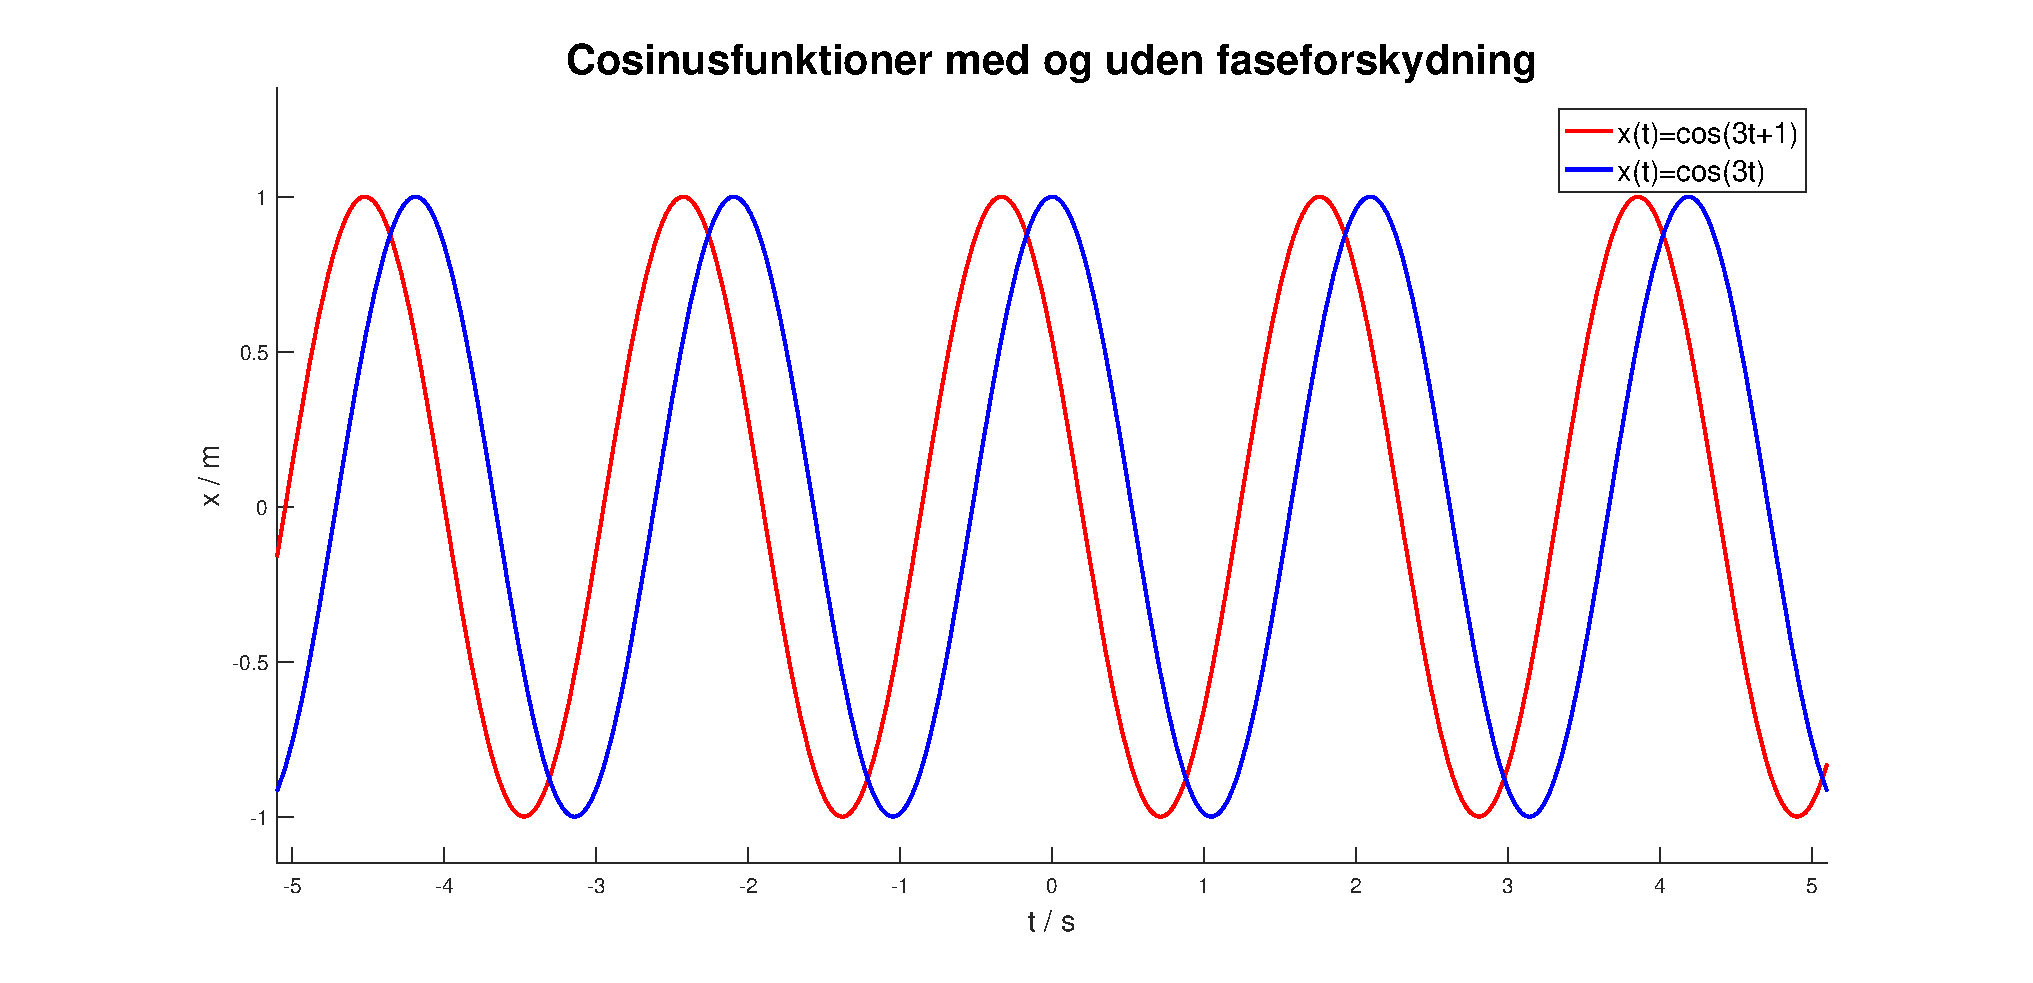
\includegraphics[width=.85\textwidth]{RotationelMekanik/Faseforskydning.eps}
\caption{Her ses to cosinusfunktioner, hvor den røde er faseforskydt i forhold til den blå med $\phi=1$. I fjedereksemplet svarer det til at tiden er startet, mens den blå er i $x=A$, og den røde er en smule foran.}
\label{fig:Faseforskydning}
\end{figure}
Det kan analogt til ligning \ref{eq:DiffLign} vises, at der tilføjes et additivt led, hvis en friktionskraft på formen $\v{f}=-b\v{v}$ medregnes
\begin{equation}
    \dd{x}{t} = -\frac{b}{m}\d{x}{t} - \frac{k}{m}x
\end{equation}
hvorved løsningen får tilføjet en eksponentiel faktor
\begin{equation}
x(t) = A\exp\left(-\frac{b}{2m}t\right)\cos\left(\omega' t + \phi\right), \qquad \omega' = \sqrt{\frac{k}{m}-\frac{b^2}{4m^2}}
\end{equation}
Harmonisk bevægelse kræver, at den resulterende kraft altid er rettet mod et hvilepunkt, der i fjederens tilfælde er loddets position i hvile. \\
For trigonometriske funktioner på følgende form
\begin{equation}
    f(x) = A\cos(B\cdot x + C)
\end{equation}
hvor $A,B,C$ er konstanter. $A$ er funktionens amplitude, og perioden er
\begin{equation}
    T = \frac{2\pi}{B}
\end{equation}
For roterende legemer kan ligning \ref{eq:N2R} bruges til at udlede bevægelsesligninger, hvor harmonisk bevægelse som det ovenstående kan forekomme nyttigt. Det kan være nyttigt at opskrive Newtons 2. lov for rotationel bevægelse på formen
\begin{equation}
    \dd{\theta}{t} = \alpha = \frac{1}{I}\sum\tau
\end{equation}
Vælges koordinatsystemet smart, kan problemet gøres mere overskueligt. Hvis der i den givne situation er en snorkraft eller normalkraft, hvis størrelse afhænger af de andre kræfter, kan origo placeres i den omtalte krafts angrebspunkt, hvorved kraftens arm og dermed kraftmomentet bliver nul. For $\v{r}_i=0$ er
\begin{equation}
    \gv{\tau}_i = \v{r}_i \times \v{F}_i = \v{0} \times \v{F}_i = \v{0}
\end{equation}